\section{Analisi dei Requisiti}
\textit{Dal 2020-12-13 al 2021-01-18}


\begin{figure}[H]
	\centering
	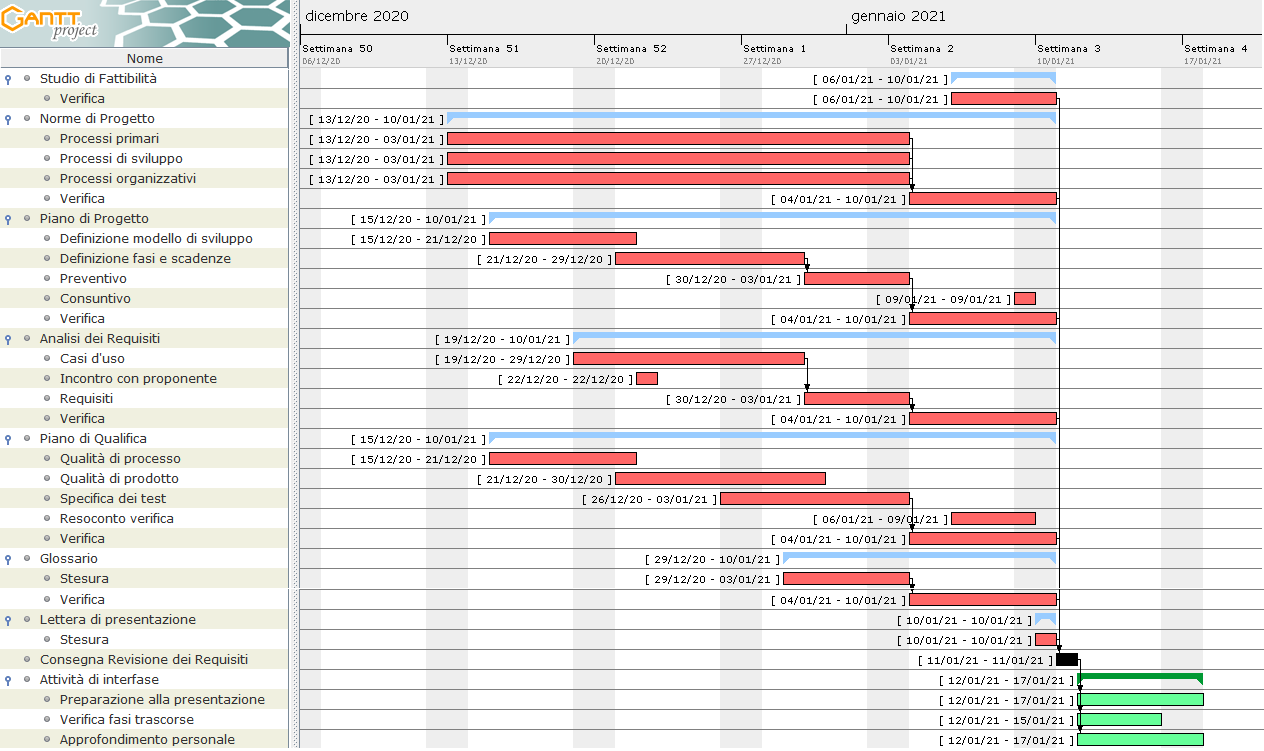
\includegraphics[scale=0.45]{res/images/02_gantt_analisi_requisiti.png}
	\caption{Diagramma di gantt\textsubscript{G} relativo alla fase\textsubscript{G} di Analisi dei Requisiti}
\end{figure}


\subsection{Periodo 1}

\subsubsection{Pianificazione preventiva}

\paragraph{Attività}

\planningTable{
	Studio di Fattibilità & Si verifica lo \textsc{Studio di Fattibilità} redatto durante la fase\textsubscript{G} di Avvio & 2 & Verificatore
\tabularnewline 
Norme di Progetto & Vengono stabilite le norme di progetto\textsubscript{G} pianificando nel dettaglio i processi primari, i processi di sviluppo e i processi organizzativi. Il documento \textsc{Norme di Progetto} viene redatto & 22 & Amministratore
\tabularnewline 
Piano di Progetto & Il Responsabile di Progetto redige il \textsc{Piano di Progetto} scandendo le fase\textsubscript{G} e i periodi secondo cui si articolerà il lavoro & 20 & Responsabile
\tabularnewline 
Analisi dei Requisiti & Uno studio approfondito del capitolato\textsubscript{G} e ne individuano i requisiti\textsubscript{G}: l'analisi si caratterizza da contatti frequenti con il proponente che fornirà supporto nella comprensione del problema. Viene completata la redazione dell'\textsc{Analisi dei Requisiti} & 50 & Analista
\tabularnewline 
Piano di Qualifica & In questa attivita\textsubscript{G} si individuano i criteri che garantiscono la qualità del prodotto. Viene redatto il \textsc{Piano di Qualifica} & 20 & Verificatore
\tabularnewline 
Glossario & Il \textsc{Glossario} conterrà i termini a cui si riterrà necessario dare definizione & 3 & Responsabile
\tabularnewline 
Verifica dei documenti & Quest'attività si concentra nella settimana che precede la presentazione e ha l'obiettivo di verificare e certificare la qualità di tutti i documenti prodotti & 23 & Verificatore
\tabularnewline 
Lettera di Presentazione & Avviene la stesura della lettera con cui il gruppo si candida alla Revisione dei Requisiti & 1 & Responsabile
\tabularnewline 
\caption{Pianificazione preventiva - Analisi dei Requisiti - Periodo 1}
}


\paragraph{Preventivo}

\smallPreventivoTable{
	Responsabile & 24 & 720\\ 
Verificatore & 45 & 675\\ 
Analista & 50 & 1250\\ 
Amministratore & 22 & 440\\ 
Programmatore & 0 & 0\\ 
Progettista & 0 & 0\\ 
\hlinetable 
\textbf{Totale} & \textbf{141} & \textbf{3085}\\ 
\end{tabular} 
\caption{Preventivo - Analisi dei Requisiti - Periodo 1}
}


\subsubsection{Riscontro di fine periodo}


\paragraph{Consuntivo orario ed economico}


\paragraph{Preventivo a finire}



\subsection{Periodo 2}

\subsubsection{Pianificazione preventiva}

\paragraph{Attività}

\planningTable{
	Preparazione alla presentazione & Viene preparato il materiale necessario alla presentazione. & 5 & Amministratore
\tabularnewline 
Verifica dei macro periodi precedenti & Il gruppo si vede coinvolto in un confronto dal quale vorranno emergere le criticità riscontrate nel macro periodo\textsubscript{G} trascorso, al fine di migliorare lo svolgimento dei periodi successivi. & 1 & Responsabile
\tabularnewline 
Approfondimento personale & Ogni membro del gruppo spende alcune ore per formare e consolidare una conoscenza di base degli strumenti e tecniche da impiegare nel periodo\textsubscript{G} successivo. & 4 & Analista
\tabularnewline 
\caption{Pianificazione preventiva - Analisi dei Requisiti - Periodo 1}
}



\paragraph{Preventivo}

\smallPreventivoTable{
	Responsabile & 1 & 30\\ 
Verificatore & 0 & 0\\ 
Analista & 4 & 100\\ 
Amministratore & 5 & 100\\ 
Programmatore & 0 & 0\\ 
Progettista & 0 & 0\\ 
\hlinetable 
\textbf{Totale} & \textbf{10} & \textbf{230}\\ 
\end{tabular} 
\caption{Preventivo - Analisi dei Requisiti - Periodo 1}
}

\subsubsection{Riscontro di fine periodo}


\paragraph{Consuntivo orario ed economico}


\paragraph{Preventivo a finire}

\pafTable{
	Avvio & 1 & Consuntivo & 
\tabularnewline
Analisi dei Requisiti & 1 & Consuntivo & 
\tabularnewline
Analisi dei Requisiti & 2 & Consuntivo & 
\tabularnewline
Progettazione Architetturale & 1 & Preventivo di periodo & 
\tabularnewline
Progettazione Architetturale & 2 & Preventivo & 2414
\tabularnewline
Progettazione Architetturale & 3 & Preventivo & 280
\tabularnewline
Progettazione di Dettaglio e Codifica & 1 & Preventivo & 1270
\tabularnewline
Progettazione di Dettaglio e Codifica & 2 & Preventivo & 4097
\tabularnewline
Progettazione di Dettaglio e Codifica & 3 & Preventivo & 258
\tabularnewline
Validazione e Collaudo & 1 & Preventivo & 220
\tabularnewline
Validazione e Collaudo & 2 & Preventivo & 2145
\tabularnewline
Validazione e Collaudo & 3 & Preventivo & 60
\tabularnewline
\textbf{Totale} & \textbf{} & \textbf{} & \textbf{10744}
\tabularnewline
\textbf{Totale rendicontato} & \textbf{} & \textbf{} & \textbf{10744}
\tabularnewline
\caption{Preventivo a finire - Analisi dei Requisiti - Periodo 2}
}